\documentclass[11pt,b5paper]{memoir} % or even: book | or the koma classes: scrreprt, scrbook
% or for a small thesis 'article' or the corresponding 'scrartcl'
%\usepackage{microtype}
%\usepackage[<encoding>]{fontenc} % probabilly: T1
\usepackage{amsmath}
% split equations with \begin{multline} ... \end{multline}
%\allowdisplaybreaks % Page breaks ?  (\begingroup  \endgroup)
\usepackage{amssymb}
\usepackage{bm}
\usepackage{xcolor}
\usepackage[utf8]{inputenc} % probabilly: utf8
%\usepackage{palatino} % just as a matter of taste
\usepackage[english]{babel}
\usepackage{lmodern}
\usepackage{geometry}
\geometry{top = 30mm}
%\usepackage{csquotes} % probabilly with the option: autostyle=true
\usepackage{ellipsis}
%\usepackage{natbib} % or biblatex
\usepackage{graphicx}
%\graphicspath{ {images/} } % or whatever your "images"-directory is
%\usepackage{todonotes} % or fixme
%\usepackage[acronym,toc]{glossaries}
\usepackage{pdfpages}
%\usepackage{setspace}


\usepackage{dsfont}

%\usepackage[toc,page]{appendix}
%

\usepackage{fancyhdr}
\usepackage{emptypage}
\usepackage{hyperref}
\usepackage[square,numbers,sort&compress,comma]{natbib}
%\setcitestyle{square,numbers,sort&compress,comma}

%\makeglossaries
%\newacronym{xo}{XO}{exchange-only}

\setcounter{tocdepth}{2}
\setcounter{secnumdepth}{2}

%\bibliographystyle{apsrev}
\bibliographystyle{aipnum4-1}
%\bibliographystyle{plainnat}
%\bibliographystyle{unsrtnat}


%\hypersetup{hidelinks}

\hypersetup{colorlinks=true,
linkcolor=blue,
citecolor=blue,
urlcolor=blue,
filecolor=black
%hidelinks
}


%\renewcommand{\headrulewidth}{0pt}
%\pagestyle{fancy}
%\fancyhf{}
%\fancyhead[LE,RO]{\thepage}
%\fancyhead[RE]{\thechapter\chaptername}
%\fancyhead[LO]{\thesection}

\renewcommand{\chaptermark}[1]{%
\markboth{\MakeUppercase{\thechapter .\ #1}}{}}

%\fancyhead[LE,RO]{\textsl{\rightmark}}
%\fancyhead[LO,RE]{\textsl{\leftmark}}
%\fancyfoot[C]{\thepage}





\newcommand{\ua}{\uparrow}
\newcommand{\da}{\downarrow}
\newcommand{\bra}[1]{\left\langle #1\right|}
\newcommand{\ket}[1]{|{#1}\rangle}
\newcommand{\braket}[2]{\langle #1 | #2 \rangle}
\newcommand{\bmk}[3]{\langle #1 | #2 | #3 \rangle}

\newcommand{\vk}{\mathbf{k}}
\newcommand{\vr}{\mathbf{r}}
\newcommand{\vR}{\mathbf{R}}

\newcommand{\comm}[2]{\left[  #1, #2 \right]}
\newcommand{\commh}[2]{\left[ #1, #2 \right]}


\newcommand{\suudd}{\left| \uparrow \uparrow S_m \downarrow \downarrow \right\rangle}
\newcommand{\sudud}{\left| \uparrow \downarrow S_m \uparrow \downarrow \right\rangle}
\newcommand{\sdudu}{\left| \downarrow \uparrow S_m \downarrow \uparrow \right\rangle}
\newcommand{\sdduu}{\left| \downarrow \downarrow S_m \uparrow \uparrow \right\rangle}
\newcommand{\sduud}{\left| \downarrow \uparrow S_m \uparrow \downarrow \right\rangle}
\newcommand{\suddu}{\left| \uparrow \downarrow S_m \downarrow \uparrow \right\rangle}

\newcommand{\uuuu}{\left| \uparrow \uparrow \uparrow \uparrow \right\rangle}
\newcommand{\uuud}{\left| \uparrow \uparrow \uparrow \downarrow \right\rangle}
\newcommand{\uudu}{\left| \uparrow \uparrow \downarrow \uparrow \right\rangle}
\newcommand{\uudd}{\left| \uparrow \uparrow \downarrow \downarrow \right\rangle}
\newcommand{\uduu}{\left| \uparrow \downarrow \uparrow \uparrow \right\rangle}
\newcommand{\udud}{\left| \uparrow \downarrow \uparrow \downarrow \right\rangle}
\newcommand{\uddu}{\left| \uparrow \downarrow \downarrow \uparrow \right\rangle}
\newcommand{\uddd}{\left| \uparrow \downarrow \downarrow \downarrow \right\rangle}
\newcommand{\duuu}{\left| \downarrow \uparrow \uparrow \uparrow \right\rangle}
\newcommand{\duud}{\left| \downarrow \uparrow \uparrow \downarrow \right\rangle}
\newcommand{\dudu}{\left| \downarrow \uparrow \downarrow \uparrow \right\rangle}
\newcommand{\dudd}{\left| \downarrow \uparrow \downarrow \downarrow \right\rangle}
\newcommand{\dduu}{\left| \downarrow \downarrow \uparrow \uparrow \right\rangle}
\newcommand{\ddud}{\left| \downarrow \downarrow \uparrow \downarrow \right\rangle}
\newcommand{\dddu}{\left| \downarrow \downarrow \downarrow \uparrow \right\rangle}
\newcommand{\dddd}{\left| \downarrow \downarrow \downarrow \downarrow \right\rangle}

\newcommand{\uuu}{\left| \uparrow \uparrow \uparrow \right\rangle}
\newcommand{\uud}{\left| \uparrow \uparrow \downarrow \right\rangle}
\newcommand{\udu}{\left| \uparrow \downarrow \uparrow \right\rangle}
\newcommand{\udd}{\left| \uparrow \downarrow \downarrow \right\rangle}
\newcommand{\duu}{\left| \downarrow \uparrow \uparrow \right\rangle}
\newcommand{\dud}{\left| \downarrow \uparrow \downarrow \right\rangle}
\newcommand{\ddu}{\left| \downarrow \downarrow \uparrow \right\rangle}
\newcommand{\ddd}{\left| \downarrow \downarrow \downarrow \right\rangle}

\newcommand{\uu}{\left| \uparrow \uparrow  \right\rangle}
\newcommand{\ud}{\left| \uparrow \downarrow \right\rangle}
\newcommand{\du}{\left| \downarrow \uparrow \right\rangle}
\newcommand{\dd}{\left| \downarrow \downarrow \right\rangle}
\newcommand{\sing}{\left| S_{02} \right\rangle}


\newcommand{\cmt}[1]{{\color{red}(#1)}}
\newcommand{\todo}[1]{\textit{\color{gray}#1}}
\renewcommand{\cs}{{\color{blue}[Citation needed]}}
%\newcommand{\todo}[1]{}



\definecolor{chaptercolor}{gray}{0.8}


\usepackage{tikz, blindtext}
\makechapterstyle{box}{
  \renewcommand*{\printchaptername}{}
%  \renewcommand*{\chapnumfont}{\fontsize{4cm}{4cm}\selectfont\sffamily\Huge\bfseries}
  \renewcommand*{\printchapternum}{
    \flushright%
%    \chapnumfont%
    {\fontsize{4cm}{4cm}\selectfont\fontfamily{qtm}\bfseries%\sffamily\bfseries%
    {\color{chaptercolor}%
    \thechapter}}%
  }
  \renewcommand*{\chaptitlefont}{\normalfont\Huge\bfseries}
  \renewcommand*{\printchaptertitle}[1]{\flushright\chaptitlefont##1}
}
\chapterstyle{box}



\author{Arnau Sala Cadellans}
\title{Exchange-only, nuclear spin-free qubits in semiconductor quantum dots}
%\date{\today}
\date{Trondheim, July 13, 2020}



\begin{document}
% roman numbering in the table of contents section

\pagenumbering{roman}
%\maketitle

\clearpage\maketitle
\thispagestyle{empty}



%\printglossary 

%\setcounter{page}{1}
\chapter*{Abstract}\noindent
This is a \textsc{latex} template intended for academic theses, and was put together by \href{https://github.com/jabirali}{Jabir Ali Ouassou} while preparing his PhD dissertation.
The template itself is released under a Creative Commons Attribution licence (\href{https://creativecommons.org/licenses/by/4.0/}{\textsc{cc by 4.0}}).
This basically means that you are free to use the template for any purpose as long as you give appropriate credit.

The template bundles the \href{https://github.com/libertinus-fonts/libertinus}{Libertinus fonts}, which is used for all regular text and mathematics, and the \href{https://ctan.org/tex-archive/fonts/urw/classico}{\textsc{urw} classico} fonts, which are used for chapter and section headings.
The former is available under the Open Font Licence (\textsc{sil ofl 1.1}), and is free for both private and commercial use.
The latter is available under the Aladdin Free Public Licence (\textsc{afpl}), and is only free for non-commercial use.
If commercial use is of importance, a suitable replacement for \textsc{urw} classico would be the Libertinus Sans fonts, which are also bundled with the template.

Note that this template relies on \textsc{lualatex} for \eg font customization, and on \textsc{bibtex} for reference handling.
For command-line users, the easiest way to compile the document is to run \texttt{latexmk -lualatex thesis.tex}.
If using an \textsc{ide}, please check the program settings for how to enable compilation with \textsc{lualatex} and \textsc{bibtex}.
The template is based on the \textsc{koma-script} book class (\texttt{scrbook}), so for further customization of the template, please check out \href{https://ctan.org/pkg/koma-script}{their documentation}.

The template does not include a title page.
This is because the style requirements typically varies between universities, and many institutions will anyway autogenerate a titlepage upon thesis submission.

\chapter*{Preface}\noindent

This thesis is submitted in partial satisfaction of the requirements of the degree Philosophiae Doctor (PhD) at the
Norwegian University of Science and Technology, in Trondheim Norway.

The work that this thesis presents started in September 2015 and ended in early spring 2021 at the
\href{https://www.ntnu.edu/quspin/center-for-quantum-spintronics}{Center for Quantum Spintronics (\textsc{QuSpin})}, \textsc{NTNU}. During this time, one
year of accumulated time was dedicated to teaching duties at the Department of Physics, and half a year
was devoted to completion of courses (30 ECTS) as pr. the requirements of the degree.
The research was supervised by
Prof. Asle Sudb{\o} as main supervisor, and Prof. Jacob Linder as co-supervisor.

Computation-time was granted at the \textsc{Vilje} and \textsc{Fram} supercomputers through the UNINETT $\int$igma$2$ e-infrastructure. The code was written in
the \href{https://julialang.org/}{\textsc{Julia}} programming language. The figures and plots were produced by the use of \textsc{Julia} and
\href{https://inkscape.org/}{\textsc{Inkscape}}.

\vspace{2cm}

\noindent Fredrik Nicolai Krohg\\
Oslo, March 2021


\chapter*{Acknowledgments\label{sec:ack}}
\addcontentsline{toc}{chapter}{Acknowledgments}

First of all I want to start by thanking my supervisor Jeroen Danon. Not only for introducing me to this fascinating field, but also for his guidance, good advice and for making me see the light on my darkest (research-wise) moments. Working with you has been a pleasant experience.

I also want to thank my coauthor and colleague J{\o}rgen Holme Qvist. It has been a pleasure to work with you.

During the last four years I have met wonderful people and great friends, here at QuSpin and beyond the outer rim of the university. I want to thank, without a particular order Longfei, Martin, Andreas, Morten, Vetle, {\O}yvind, Jonas, Payel, Sol, Justin, and well... many others.
%
Some people deserve a special consideration, though. These are the ones I spent most time with, and those with whom I have had the most interesting physics (or not) discussions. Thank you Lina, Jonas Ghini, Matthias, Max, Vasil, Akash, Atousa, Eirik and H{\aa}vard.
%
I need also thank Even and Nicolai for all the Fridays (and some Mondays) at ``beatz''. Thank you Even and Vasil also for all the lunch-over-Teams we have had together during the home-office period.

And from outside QuSpin I cannot forget about Tonje, May Lise, Corinna, Tengzhi, Sophia, and most specially Nastasia. You have been one of my greatest friends and I am very grateful for all the hikes, dinners, drinks, movies, chess matches, (infinitely) long talks, and everything we have done together.


I also want to thank my family and most especially my brother Xavier, with whom I have spent some of my most memorable moments. Next time you get stuck in a foreign country call me!


\cleardoublepage

% Table of contents :  it is a good idea to include this into your thesis
%\tableofcontents*
\begin{KeepFromToc}
  \tableofcontents
\end{KeepFromToc}
\cleardoublepage

% The following list of figures and list of tables are optional. Remove the comments if needed
%\listoffigures
%\newpage

%\listoftables
%\newpage

% in the main part of the document use standard Arabic numbers. Page counter resets to 1.
\pagenumbering{arabic}

\chapter{Introduction\label{sec:intro}}

\hfill%
\begin{minipage}{0.85\textwidth}
\em
%\hfill ``Quantum computers make Internet faster''.
%
%\hfill ---My mom.
This chapter is only an appetizer. We will not go into details here, but we will introduce some concepts that we use in the rest of this thesis.
\end{minipage}\\
\vspace{3ex}





\section{Quantum computation}

It seems that with a computer we can calculate anything: We just need enough memory and enough time. Yet every time we write a code to run some calculations we have to think how to optimize it because we never have enough memory or time.
%
A quantum computer is not much different. We will not be able to solve \textit{any} problem instantaneously with a quantum laptop (if such a thing ever exists), but if we are smart enough we can use the extra toolbox that quantum mechanics provide to solve some problems very efficiently.

Take for example Shor's algorithm. Everyone has studied (or heard about) this algorithm in undergraduate courses.
%
If you want to factorize a large number $N$ in your laptop you can take the naive approach and try dividing it by all prime numbers between 2 and $\sqrt N$, but that can take some time. There are more efficient algorithms to do that, but in the best case the computational time that takes to solve this problem scales exponentially with the number of digits of $N$ and becomes intractable for large enough $N$~\cite{Nielsen2010}.
%
Shor's algorithm~\cite{Shor1994,Ekert1996,Nielsen2010} may look inefficient too because it requires calculating Fourier transforms, which are typically slow (and also require a large amount of memory). But there is a twist: In a quantum computer we can calculate Fourier transforms in a polynomial time rather than exponential, as is the case in classic computers.
%
Shor's algorithm can thus be implemented in a quantum computer to solve the problem of factorization of large numbers efficiently in a polynomial time.




\begin{figure}
  \centering
  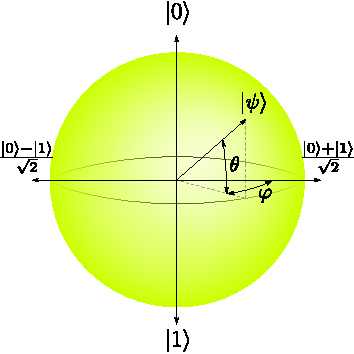
\includegraphics[scale=1]{intro/figs/bloch.pdf}
  \caption{ A quantum state $\ket\psi$ is represented as a point in the surface of the Bloch sphere. The angle theta contains information about the overlap between the state $\ket\psi$ and the basis states $\ket 0$ and $\ket 1$, whereas the angle $\varphi$ describes a phase. \label{fig1:bloch}}
\end{figure}

We will not go into details about quantum computation and quantum algorithms.
%
This is just an example of the powerful capabilities of a quantum computer, but it is not in the scope of this thesis to convince anyone why we need quantum computers and what can they do for us. A quick Google search will already mention some of its applications in internet security, research, etc.
%
We will instead focus on the most essential part of quantum computers: the qubit. A qubit is a quantum bit. It is the analog of a bit in a classic computer but it is not limited to be either in the state 0 or 1. A qubit can be in any quantum superposition of the states $\ket 0$ and $\ket 1$. Qubits are often represented as points in the surface of a sphere: the Bloch sphere. Indeed, any qubit can be expressed as
\begin{align}
\ket{\psi (\theta,\varphi)}  = {}&{} \cos\frac{\theta}{2}\ket 0 + e^{i\varphi} \sin\frac{\theta}{2}\ket 1,
\end{align}
up to an overall phase,
where $\theta$ and $\varphi$ are the polar and azimuthal angles in the Bloch sphere of Fig.~\ref{fig1:bloch}. The states $\ket 0$ and $\ket 1$ denote the north and south poles, respectively, of the sphere.





A qubit is thus a quantum mechanical two-level system, and we need to find a physical implementation of this two-level system if we want to create a quantum computer. When one thinks about two-level quantum systems the first thing that comes to mind is probably the spin of an electron. That is text-book physics. And that is (maybe) what Daniel Loss and David DiVincenzo thought when they wrote their seminal paper on quantum computation using quantum dots~\cite{Loss1998}.


The idea is very simple: If we can localize one electron and manipulate its spin, we can use the spin states $\ket\ua$ and $\ket \da$ as the qubit states. We also need a mechanism to initialize the qubit into any desired quantum state, read out the output state after running a quantum algorithm and we must also be able to couple this qubit to, at least, another qubit to perform two-qubit gates~\cite{DiVincenzo2000a,Nielsen2010}. In Ref.~\cite{Loss1998} the authors address all these issues and propose to localize the electrons in \textit{quantum dots}.



\section{Quantum dots}

\begin{figure}
  \centering
  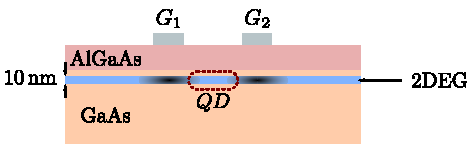
\includegraphics[scale=1]{intro/figs/2deg.pdf}
  \caption{ A 2DEG is formed e.g., close to the interface between a GaAs/AlGaAs heterojunction~\cite{Hanson2007}. It consists of a thin layer ($\sim 10$nm) where electrons can have a high mobility. Top gates ($G_{1}$ and $G_{2}$), lithographically grown, can create a depletion zone in the 2DEG (dark areas), isolating a small region where we can trap one or a few excess electrons (the region enclosed by the dashed red curve). This is a quantum dot.  \label{fig1:2deg}}
\end{figure}

A quantum dot is a potential well that can trap one or a few electrons (or holes). They are typically fabricated in semiconductors, in a two-dimensional electron gas (2DEG). We can think of a 2DEG as a surface in a semiconductor where electrons occupy the conduction band and, thus, can move relatively freely. A 2DEG can be created in Si MOSFETs, in Si/Ge heterostructures, in GaAs/AlGaAs, etc, and in all cases the electrons are confined in a triangular potential along the $z$ direction only, but are unbounded in the $x$-$y$ plane~\cite{Hanson2007,Zwanenburg2013}.


On top of the heterostructure we can put metallic gates. These can be used to apply a localized electric field and create a depletion zone in the 2DEG (see Fig.~\ref{fig1:2deg}). These depletion zones can be engineered to create a whole closed area in the 2DEG where we can trap one or a few electrons. This artificial potential well is a quantum dot.

Once we have a quantum dot we can couple it to a reservoir (by letting electrons tunnel in and out of the quantum dot) and trap one electron. Then we can use the spin of this localized electron for quantum computation.




\section{Making a spin qubit (using quantum dots)}



To understand how a quantum dot-based spin qubit works it is better to see a top view of the device. Fig.~\ref{fig1:2qd} shows a schematic illustration of a system composed of two quantum dots.

\begin{figure}
  \centering
  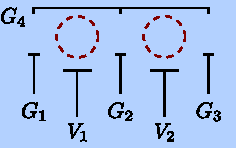
\includegraphics[scale=1]{intro/figs/fig2qd.pdf}
  \caption{ Negative voltages applied to the metallic gates $G_1$, $G_2$, $G_3$ and $G_4$ create a depletion zone in the 2DEG (blue surface). This results in two small isolated islands, the quantum dots, where electrons can be trapped (red circles). The electrochemical potential in the dots can be controlled by the gates $V_1$ and $V_2$. \label{fig1:2qd}}
\end{figure}
The blue surface represents the 2DEG. On top of the device several metallic gates can be individually addressed to create and manipulate the quantum dots: By applying a negative potential on the gates $G_i$, the resulting electric field creates a depletion zone on the 2DEG where electrons are not allowed and a small island where the electrons can be trapped. In Fig.~\ref{fig1:2qd} we show two of such islands, indicated by red dashed circles. These are the quantum dots. We can control the coupling between the two dots by detuning of the gate $G_2$. The gates $G_1$ and $G_3$ can be used to allow electrons in and out of the quantum dots, while the gates $V_1$ and $V_2$ control the electrochemical potential in the dots.

If we now trap one electron in each of the dots we can control its spin with magnetic fields. In fact, with such a simple device, composed of only two quantum dots, it is possible to implement a quantum algorithm~\cite{Watson2018}.

But in this thesis we are not interested in single-spin qubits. The goal of our project is to study decoherence mechanisms in exchange-only spin qubits and mitigate their effects.



\include{spinqubits/spinqubits}
\include{xoso/xoso}
\include{htxoso/htxoso}
\include{leakage/leakage}
\include{edsr/edsr}
\include{app/appSW}



\chapter*{Epilogue\label{sec:epi}}
\addcontentsline{toc}{chapter}{Epilogue}

%Why quantum dots? Certainly there are many reasons to devote a PhD to the study of quantum dots, and I will mention them below in the appropriate chapters, but let me start with my personal motivation for doing this project.
Why quantum dots? Certainly there are many reasons to devote a PhD to the study of quantum dots (and I hope I have already given you some) but let me state now my personal motivation for doing this project.
I would lie if I say that I believed from the very beginning that quantum dots are the future of quantum computation or that large-scale quantum computation is possible \textit{only} with quantum dots. But quantum dots \textit{are} a physical system capable of quantum computation. It is a new---twenty-years-old new---thing. There are plenty of phenomena to be discovered and understood. They possess unique features that other systems lack... And it is fun!
Don't get me wrong. I am not the kind of physicist who enjoys research for research. I need a motivation, a purpose. I need to know that my research will have a practical use (and, if possible, an impact on society). I am not against pure research. I understand that it is utterly necessary, but it is not what makes me tick. In this regard quantum dots provided me with the motivation that I so much needed to devote four years of my life closed in an office Monday to Sunday instead of taking my skis and getting lost in the snow-covered mountains of Tr{\o}ndelag.

\vspace{1cm}
\begin{flushright}
Arnau Sala\\
Trondheim, Norway,\\
July 2020
\end{flushright}

%These have been four wonderful years and I have enjoyed each and every day.



\bibliography{refs}









%% The papers

\cleardoublepage
\thispagestyle{empty}
\begin{vplace}[0.7]
\begin{center}
%\linespread{2.0}
\textbf{\huge Paper I}\\
\vspace{3ex}
\textbf{Arnau Sala and Jeroen Danon}\\
\vspace{2ex}
\textit{Exchange-only singlet-only spin qubit}\\
\vspace{2ex}
Physical Review B, \textbf{95}, 241303(R) (2017)
\end{center}
\end{vplace}
\cleardoublepage
\includepdf[pages=-]{papers/Paper_I.pdf}


\cleardoublepage
\thispagestyle{empty}
\begin{vplace}[0.7]
\begin{center}
\textbf{\huge Paper II}\\
\vspace{4ex}
\textbf{Arnau Sala and Jeroen Danon}\\
\vspace{2ex}
\textit{Leakage and dephasing in $^{28}$Si-based exchange-only spin qubits}\\
\vspace{2ex}
Physical Review B, \textbf{98}, 245409 (2018)
\end{center}
\end{vplace}
\cleardoublepage
\includepdf[pages=-]{papers/Paper_II.pdf}


\cleardoublepage
\thispagestyle{empty}
\begin{vplace}[0.7]
\begin{center}
\textbf{\huge Paper III}\\
\vspace{4ex}
\textbf{Arnau Sala, J{\o}rgen Holme Qvist and Jeroen Danon}\\
\vspace{2ex}
\textit{Highly tunable exchange-only singlet-only qubit in a GaAs \\triple quantum dot}\\
\vspace{2ex}
Physical Review Research, \textbf{2}, 012062(R) (2020)
\end{center}
\end{vplace}
\cleardoublepage
\includepdf[pages=-]{papers/Paper_III.pdf}

\end{document}



